\documentclass[12pt]{article}
\def\activityid{F10-U-v3}\usepackage[letterpaper,margin=.65in,top=.60in,bottom=.65in]{geometry}
\usepackage[T1]{fontenc}
\usepackage[default]{sourcesanspro}
\usepackage{microtype,tikz,array,tabularx,fancyhdr,amsmath,amssymb}
\usepackage[hidelinks]{hyperref}
\usetikzlibrary{calc,arrows.meta}
\setlength{\parindent}{0pt}\setlength{\parskip}{7pt}
\setlength{\headheight}{0pt}\setlength{\footskip}{26pt}\setlength{\emergencystretch}{2em}
\pagestyle{fancy}\fancyhf{}\renewcommand{\headrulewidth}{0pt}\renewcommand{\footrulewidth}{.4pt}
\fancyfoot[L]{\scriptsize Bellingham Math Circle / Week 10 / \activityid}
\fancyfoot[R]{\scriptsize \thepage}
\definecolor{ink}{gray}{.12}\definecolor{soft}{gray}{.95}\color{ink}
\newcommand{\PageTitle}[2]{{\fontsize{10}{12}\selectfont\bfseries WEEK 10\quad ROUTE LAB\hfill #1\par}\vspace{3pt}{\fontsize{26}{29}\selectfont\bfseries #2\par}\vspace{2pt}}
\newcommand{\Subhead}[1]{\par\vspace{3pt}{\large\bfseries #1}\par}
\newcommand{\RuleBox}[1]{\par\begingroup\setlength{\fboxsep}{8pt}\colorbox{soft}{\parbox{\dimexpr\linewidth-16pt\relax}{#1}}\endgroup\par}
\newcommand{\WriteBox}[2]{\par\textbf{#1}\par\vspace{2pt}\begin{tikzpicture}\draw[black!40,line width=.5pt] (0,0) rectangle (\dimexpr\linewidth-.5pt\relax,#2);\end{tikzpicture}\par}
\newcommand{\RookBoard}[3]{\begin{tikzpicture}[x=#3,y=#3]\draw[step=1,black!45] (0,0) grid (#1,#2);\draw[thick] (0,0) rectangle (#1,#2);\node[font=\Large] at ({#1-.5},.5){$\star$};\draw[-{Latex},thick] (0,-.35)--(#1,-.35);\draw[-{Latex},thick] ({#1+.35},#2)--({#1+.35},0);\end{tikzpicture}}
\newcommand{\Table}[3]{\begin{tikzpicture}[x=#3,y=#3]\draw[step=1,black!25] (0,0) grid (#1,#2);\draw[thick] (0,0) rectangle (#1,#2);\fill (0,0)circle(3pt);\draw[-{Latex},very thick] (0,0)--(.7,.7);\node[below] at ({#1/2},-.1){width #1};\node[rotate=90,above] at (-.2,{#2/2}){height #2};\end{tikzpicture}}
\newcommand{\GraphNodes}{\coordinate(A)at(0,0);\coordinate(B)at(3,0);\coordinate(C)at(1.5,2.6);\coordinate(D)at(1.5,.95);}
\newcommand{\Kfour}[1]{\begin{tikzpicture}[scale=#1]\GraphNodes\draw[very thick](A)--(B)--(C)--(A)--(D)--(B) (D)--(C);\foreach \n in {A,B,C,D}{\node[circle,draw,fill=white,minimum size=22pt,font=\bfseries]at(\n){\n};}\end{tikzpicture}}
\newcommand{\House}[1]{\begin{tikzpicture}[scale=#1]\coordinate(A)at(0,0);\coordinate(B)at(3,0);\coordinate(C)at(3,2);\coordinate(D)at(0,2);\coordinate(E)at(1.5,3.3);\draw[very thick](A)--(B)--(C)--(D)--(A) (D)--(E)--(C);\foreach \n in {A,B,C,D,E}{\node[circle,draw,fill=white,minimum size=22pt,font=\bfseries]at(\n){\n};}\end{tikzpicture}}




\newcommand{\StudentPage}[1]{{\fontsize{10}{12}\selectfont\bfseries Week 10 / Route lab / #1\par}\vspace{10pt}}
\newcommand{\Problem}[2]{\par\noindent\textbf{Problem #1:} #2\par}
\newcommand{\Space}[1]{\par\begin{tikzpicture}\draw[black!35] (0,0) rectangle (\dimexpr\linewidth-.5pt\relax,#1);\end{tikzpicture}\par}
\newcommand{\Piles}[1]{\begin{center}\begin{tikzpicture}[x=1in,y=1in]\foreach \x in {0,...,#1}{\draw[black!50,rounded corners] ({\x*2.05},0) rectangle ({\x*2.05+1.8},1.3);}\end{tikzpicture}\end{center}}

\newcommand{\Triangle}[1]{\begin{tikzpicture}[scale=#1]\draw[very thick](0,0)--(2,0)--(1,1.7)--cycle;\foreach\n/\x/\y in{A/0/0,B/2/0,C/1/1.7}{\node[circle,draw,fill=white,minimum size=25pt]at(\x,\y){\n};}\end{tikzpicture}}
\newcommand{\Branch}[1]{\begin{tikzpicture}[scale=#1]\draw[very thick](0,0)--(2,0)--(1,1.7)--cycle (0,0)--(-1.2,-.8);\foreach\n/\x/\y in{A/0/0,B/2/0,C/1/1.7,D/-1.2/-.8}{\node[circle,draw,fill=white,minimum size=25pt]at(\x,\y){\n};}\end{tikzpicture}}
\newcommand{\StarGraph}[1]{\begin{tikzpicture}[scale=#1]\draw[very thick](0,0)--(0,1.5) (0,0)--(-1.5,-1) (0,0)--(1.5,-1);\foreach\n/\x/\y in{A/0/0,B/0/1.5,C/-1.5/-1,D/1.5/-1}{\node[circle,draw,fill=white,minimum size=25pt]at(\x,\y){\n};}\end{tikzpicture}}
\newcommand{\TwoLoops}[1]{\begin{tikzpicture}[scale=#1]\coordinate(A)at(0,0);\coordinate(B)at(-1.5,1.25);\coordinate(C)at(-1.5,-1.25);\coordinate(D)at(1.5,1.25);\coordinate(E)at(1.5,-1.25);\draw[very thick](A)--(B)--(C)--(A)--(D)--(E)--(A);\foreach\n in{A,B,C,D,E}{\node[circle,draw,fill=white,minimum size=22pt]at(\n){\n};}\end{tikzpicture}}
\newcommand{\WeightedGraph}[1]{\begin{tikzpicture}[scale=#1]\GraphNodes\draw[very thick](A)--node[midway,fill=white,inner sep=1.5pt]{2}(B)--node[midway,fill=white,inner sep=1.5pt]{3}(C)--node[midway,fill=white,inner sep=1.5pt]{7}(A);\draw[very thick](A)--node[midway,fill=white,inner sep=1.5pt]{1}(D)--node[midway,fill=white,inner sep=1.5pt]{6}(B) (D)--node[midway,fill=white,inner sep=1.5pt]{1}(C);\foreach\n in{A,B,C,D}{\node[circle,draw,fill=white,minimum size=22pt,font=\bfseries]at(\n){\n};}\end{tikzpicture}}

\begin{document}

\StudentPage{Grades 4--5}
\Problem{1}{Try to use every line once without jumping. Revisiting a dot is allowed. Mark used lines with counters. Try the house, then the triangle with center D. Choose two different starting dots on each. Record a complete route, or your attempted route and unused lines.}
\begin{center}\House{1.0}\hspace{.6in}\Kfour{1.0}\end{center}
\begin{center}\renewcommand{\arraystretch}{2.2}\begin{tabular}{c|c|p{2.6in}|p{1.25in}}Map&Start&Route&Unused lines\\\hline House&&&\\House&&&\\Triangle&&&\\Triangle&&&\end{tabular}\end{center}
\Problem{2}{Count each dot's incident lines, called its degree. Circle the odd-degree dots. Choose your complete house route and pair the arrival/departure lines at each internal visit. Record the dots with one unpaired line.}
\Space{1in}
\newpage
\StudentPage{Grades 4--5}
\Problem{3}{Walk A--B--C--A and mark those roads used. Walk the remaining loop A--D--E--A. Write each loop on a paper strip. Join the strips at A to make one route using all six roads. Record and trace the joined route.}
\begin{center}\TwoLoops{1.4}\end{center}
\Space{.55in}
\Problem{4}{The map below adds a loop at B. Start with your route from Problem 3, then insert B--F--G--B at a visit to B. Record the joined route and check every road is used once. Count the degree at B before and after the new loop.}
\begin{center}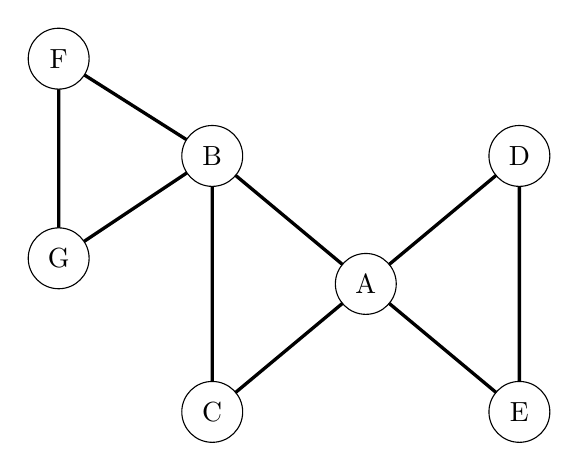
\begin{tikzpicture}[scale=1.3]\coordinate(A)at(0,0);\coordinate(B)at(-1.5,1.25);\coordinate(C)at(-1.5,-1.25);\coordinate(D)at(1.5,1.25);\coordinate(E)at(1.5,-1.25);\coordinate(F)at(-3,2.2);\coordinate(G)at(-3,.25);\draw[very thick](A)--(B)--(C)--(A)--(D)--(E)--(A) (B)--(F)--(G)--(B);\foreach\n in{A,B,C,D,E,F,G}{\node[circle,draw,fill=white,minimum size=22pt]at(\n){\n};}\end{tikzpicture}\end{center}
\Space{.65in}
\newpage
\StudentPage{Grades 4--5}
\Problem{5}{Now travel every road at least once and return to A. Roads may be repeated; each traversal costs 1 step. Find a route on the left map and record its visited dots. Try a different route on the right map with fewer steps, or match your best count. Mark each repeated road with an extra pencil line.}
\begin{center}\Kfour{1.25}\hspace{.8in}\Kfour{1.25}\end{center}
\begin{center}\renewcommand{\arraystretch}{2.3}\begin{tabular}{c|p{3.6in}|c}Trial&Route&Steps\\\hline1&&\\2&&\end{tabular}\end{center}
\Problem{6}{Count how many times your best route uses each road. Record the original six crossings separately from the repeats. At each dot, count all arrival and departure crossings, including repetitions. Circle any odd total.}
\begin{center}\renewcommand{\arraystretch}{2}\begin{tabular}{c|cccccc}Road&AB&AC&AD&BC&BD&CD\\\hline Times used&&&&&&\end{tabular}\end{center}
\Problem{7}{Add one extra copy of a road to a clean map. Count how many odd degrees change to even. Then add one more road copy that makes all degrees even. Record the two roads.}
\Space{.85in}
\newpage
\StudentPage{Grades 4--5}
\Problem{8}{Pair the four odd dots in each way shown. Draw a second copy of each named road on its map. Then find a closed route using every original and added road once. Record its length.}
\begin{center}\begin{tabular}{ccc}AB + CD&AC + BD&AD + BC\\\Kfour{.98}&\Kfour{.98}&\Kfour{.98}\end{tabular}\end{center}
\begin{center}\renewcommand{\arraystretch}{2.2}\begin{tabular}{c|p{3.5in}|c}Pairing&Closed route&Length\\\hline AB + CD&&\\AC + BD&&\\AD + BC&&\end{tabular}\end{center}
\Problem{9}{Now the truck may finish at a different dot. Add just one road copy to the original map below, then find a route using every original and added road once. Record its endpoints and length.}
\begin{center}\Kfour{1.05}\end{center}
\Space{.8in}
\newpage
\StudentPage{Grades 4--5}
\Problem{10}{Add three roads between these two triangles so the map is connected and all six dots have odd degree. Curve roads around other dots; a crossing without a dot is not a junction. Count the degrees. Then choose three roads to repeat so every degree becomes even. Record a closed delivery route and its length.}
\begin{center}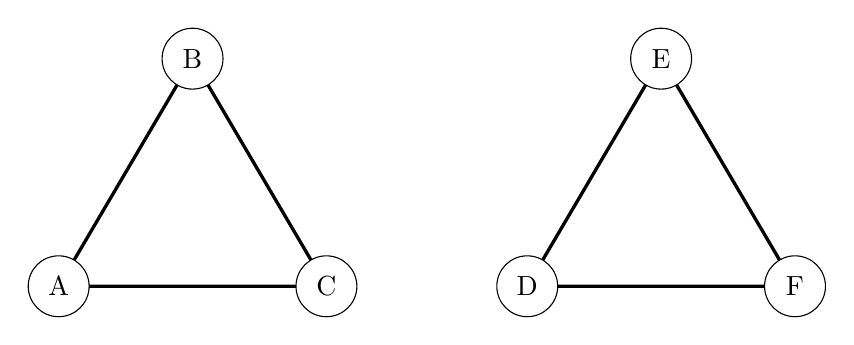
\begin{tikzpicture}[scale=1.7]\coordinate(A)at(0,0);\coordinate(B)at(1,1.7);\coordinate(C)at(2,0);\coordinate(D)at(3.5,0);\coordinate(E)at(4.5,1.7);\coordinate(F)at(5.5,0);\draw[very thick](A)--(B)--(C)--cycle (D)--(E)--(F)--cycle;\foreach\n in{A,B,C,D,E,F}{\node[circle,draw,fill=white,minimum size=22pt]at(\n){\n};}\end{tikzpicture}\end{center}
\Space{.85in}
\Problem{11}{This map also has six odd dots. Start at A, visit every road, and return to A. Mark each repeated road and record your route. Compare how many extra crossings the two maps need.}
\begin{center}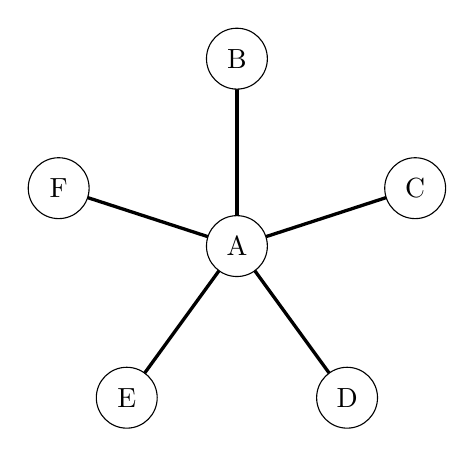
\begin{tikzpicture}[scale=1.4]\coordinate(A)at(0,0);\foreach\n/\ang in{B/90,C/18,D/-54,E/-126,F/162}{\coordinate(\n)at(\ang:1.7);\draw[very thick](A)--(\n);\node[circle,draw,fill=white,minimum size=22pt]at(\n){\n};}\node[circle,draw,fill=white,minimum size=22pt]at(A){A};\end{tikzpicture}\end{center}
\Space{.75in}

\end{document}
